\section{Methodology of DEM Parameter Identification}
\label{sec:methodology}

We now illustrate the methodology used, also shown in Fig.
\ref{fig:19methodology}.
\begin{figure}[!htb] 
\centering 
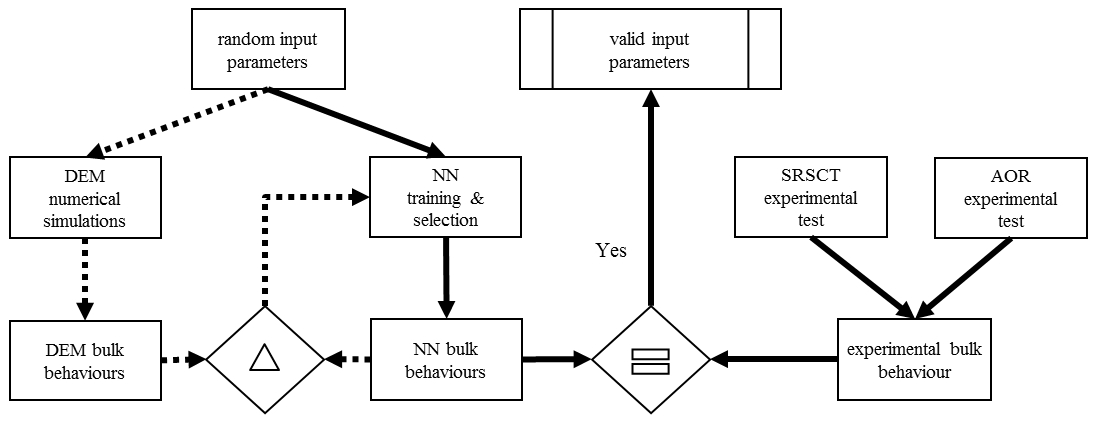
\includegraphics[width=.96\textwidth]{19methodology} 
\caption[Methodology]{Methodology. 
In the training phase (dashed lines) from the initial random input parameters
$DEM$ simulations are performed. The behaviours provided are used to train the
Neural Networks ($NN$), in a loop that continues until the difference is within
the limit ($\Delta$).
Then in the parameters' identification phase (straight
lines) we identify the valid input parameters by comparing (\textbf{=}) $NN$ and
experimental behaviours.
Further explanations in the text.
}
\label{fig:19methodology} 
\end{figure}


% \begin{figure}[htp]
%     \centering
%     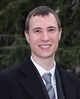
\includegraphics[width=.2\textwidth]{images/vitae/lbenvenuti}
%     \caption{OpenMP, MPI, MPI/OpenMP Hybrid runs of Box in a box testcase on 32
%     cores. The OpenMP-only run suffers from limited memory bandwidth in
%     memory-bound algorithms inside of the Modify section of the code. MPI-only has
%     low averaged runtimes for each section, but a very large Other timing, which
%     hints for a large amount of load-imbalance. Hybrid timings are a bit worse
%     on average, but because of better balancing, processes have lower wait times
%     inside of Other timing.}
% 	\label{fig:boxInBoxComparison}



% After the $DEM$ simulations the Neural
% Network ($NN$) are trained and selected. We then compare experimental and
% numerical results to identify the valid parameters.

% For simulations purposes, we also sieved the bulk to know the size distribution.
% We could then focus on the simulations. 

\subsection{Discrete element method}
\label{subsec:dem}

We decided to fix one single
contact law for all the simulations performed, see
\ref{subsec:srsctsimulation}.
The $DEM$ parameters for the Young's modulus ($E$) and the coefficient of Poisson ($\nu$) 
have been taken from the literature, see \cite{RefWorks:175} and \cite{RefWorks:176}, 
although we reduced the former to increase the time step ($\Delta t$), following
the indications of Ai et al. \cite{RefWorks:131}.
The last was between $1.29 \%$ and $1.53 \%$ of the Rayleigh time, that also
depends to the particle density ($\rho_p$).
Furthermore, we locked the size distribution, provided by experimental sieving,
see table \ref{tab:09DEMFixedinputvalues}.
In the contact law we used, 
the tangential component of the contact force between two generic particles
($F_t$) is truncated to fulfil
\begin{equation}
F_{t,ij} \leq \mu_s F_{n,ij},
 \label{eq:force_t}
\end{equation}

where $F_n$ is the normal component and $\mu_s$ is the coefficient of sliding
friction, one of the particle based $DEM$ parameter we investigated. 
Another parameter was the coefficient of rolling friction ($\mu_r$). 
For coarse not round particles is a critical parameter and describes inter-particle 
friction in medium to dense granular flows simulations. It is proportional to the 
torque counteracting the rotation of the particle. The $\mu_r$ parameter enters the 
equations according to the elasto-rolling resistance model presented by Wensrich and 
Katterfeld \cite{RefWorks:87} and Ai et al. \cite{RefWorks:131}, 
based on the work of Jiang et al. \cite{RefWorks:143}. 
The model is called $EPSD2$ in $LIGGGHTS$. This is appropriate for the one way
rolling cases as well as the cycling rolling ones.
The maximum magnitude of rolling resistance torque is (Eq. \ref{eq:trmax}):
\begin{equation}
T_{r~max} = \mu_r R_r |\tilde{F_n}| ~,
 \label{eq:trmax}
\end{equation}

where $R_r$ is the equivalent radius and $F_n$ the normal force.
The last two particle based $DEM$ parameter we investigated were the $\rho_p$
and the coefficient of restitution ($COR$), as defined by Ai. et al. \cite{RefWorks:131}.

The coefficients, $COR$, $\mu_s$, $\mu_r$,
$\rho_p$ and $dCylDp$ (the cylinder dimension, as proportion to the mean
particle diameter), as indicated in table \ref{tab:10DEMVariableinputvalues}, were constant in each simulation, but their combination differed between
simulations.
Further, $dCylDp$ was used to evaluate the wall effect, but only $~10\%$ of the
all simulations had $dCylDp$ larger than $20$ (additional information can be found in \ref{subsec:srsctsimulation}). 
The normal stress $\sigma_n$ and its
percentage during the incipient flow condition $\tau_{\%}$
varied to replicate twelve shear cell load conditions. 
The complete description of the shear cell simulations can be found in \ref{subsec:srsctsimulation}, 
while the $AoR$ simulation is presented in \ref{subsec:aorsimulation}.
A Matlab script allowed us to extract from the simulations output the numerical
bulk representative values for
each $simulation-DEM$ parameter combination:
bulk density ($\rho_b$),
coefficient of internal friction in the pre-shear phase ($\mu_{psh}$),
coefficient of internal friction in the shear phase ($\mu_{sh}$),
and angle of repose ($AoR$).
The first bulk behaviour representative value ($\rho_b$) was directly provided. 
If a simulation was performed correctly, see \ref{subsec:srsctsimulation}, we
observed a stress path as in Fig. \ref{fig:21simexample}.
First, the $\sigma_n$ was kept constant. 
Meanwhile, the coefficient of internal friction ($\mu_{ie}$) initially increased
and then reached a plateau.
The second bulk behaviour representative value ($\mu_{psh}$) was calculated as average of the $\mu_{ie}$ in this plateau.
Automatically, the $\sigma_n$ was reduced, in this example to $80 \%$ of its
initial value.
After, a second plateau started.
As average of $\mu_{ie}$ in this second plateau we obtained the third value
($\mu_{sh}$).
The stress path is
comparable to the experimental one, especially the plateaux.\\
In the $AoR$ tests the average of the repose angles provided us the fourth bulk
value, allowing us to define the numerical bulk behaviour.
\begin{figure}[htp] \centering
    \begin{subfigure}[b]{2cm}
        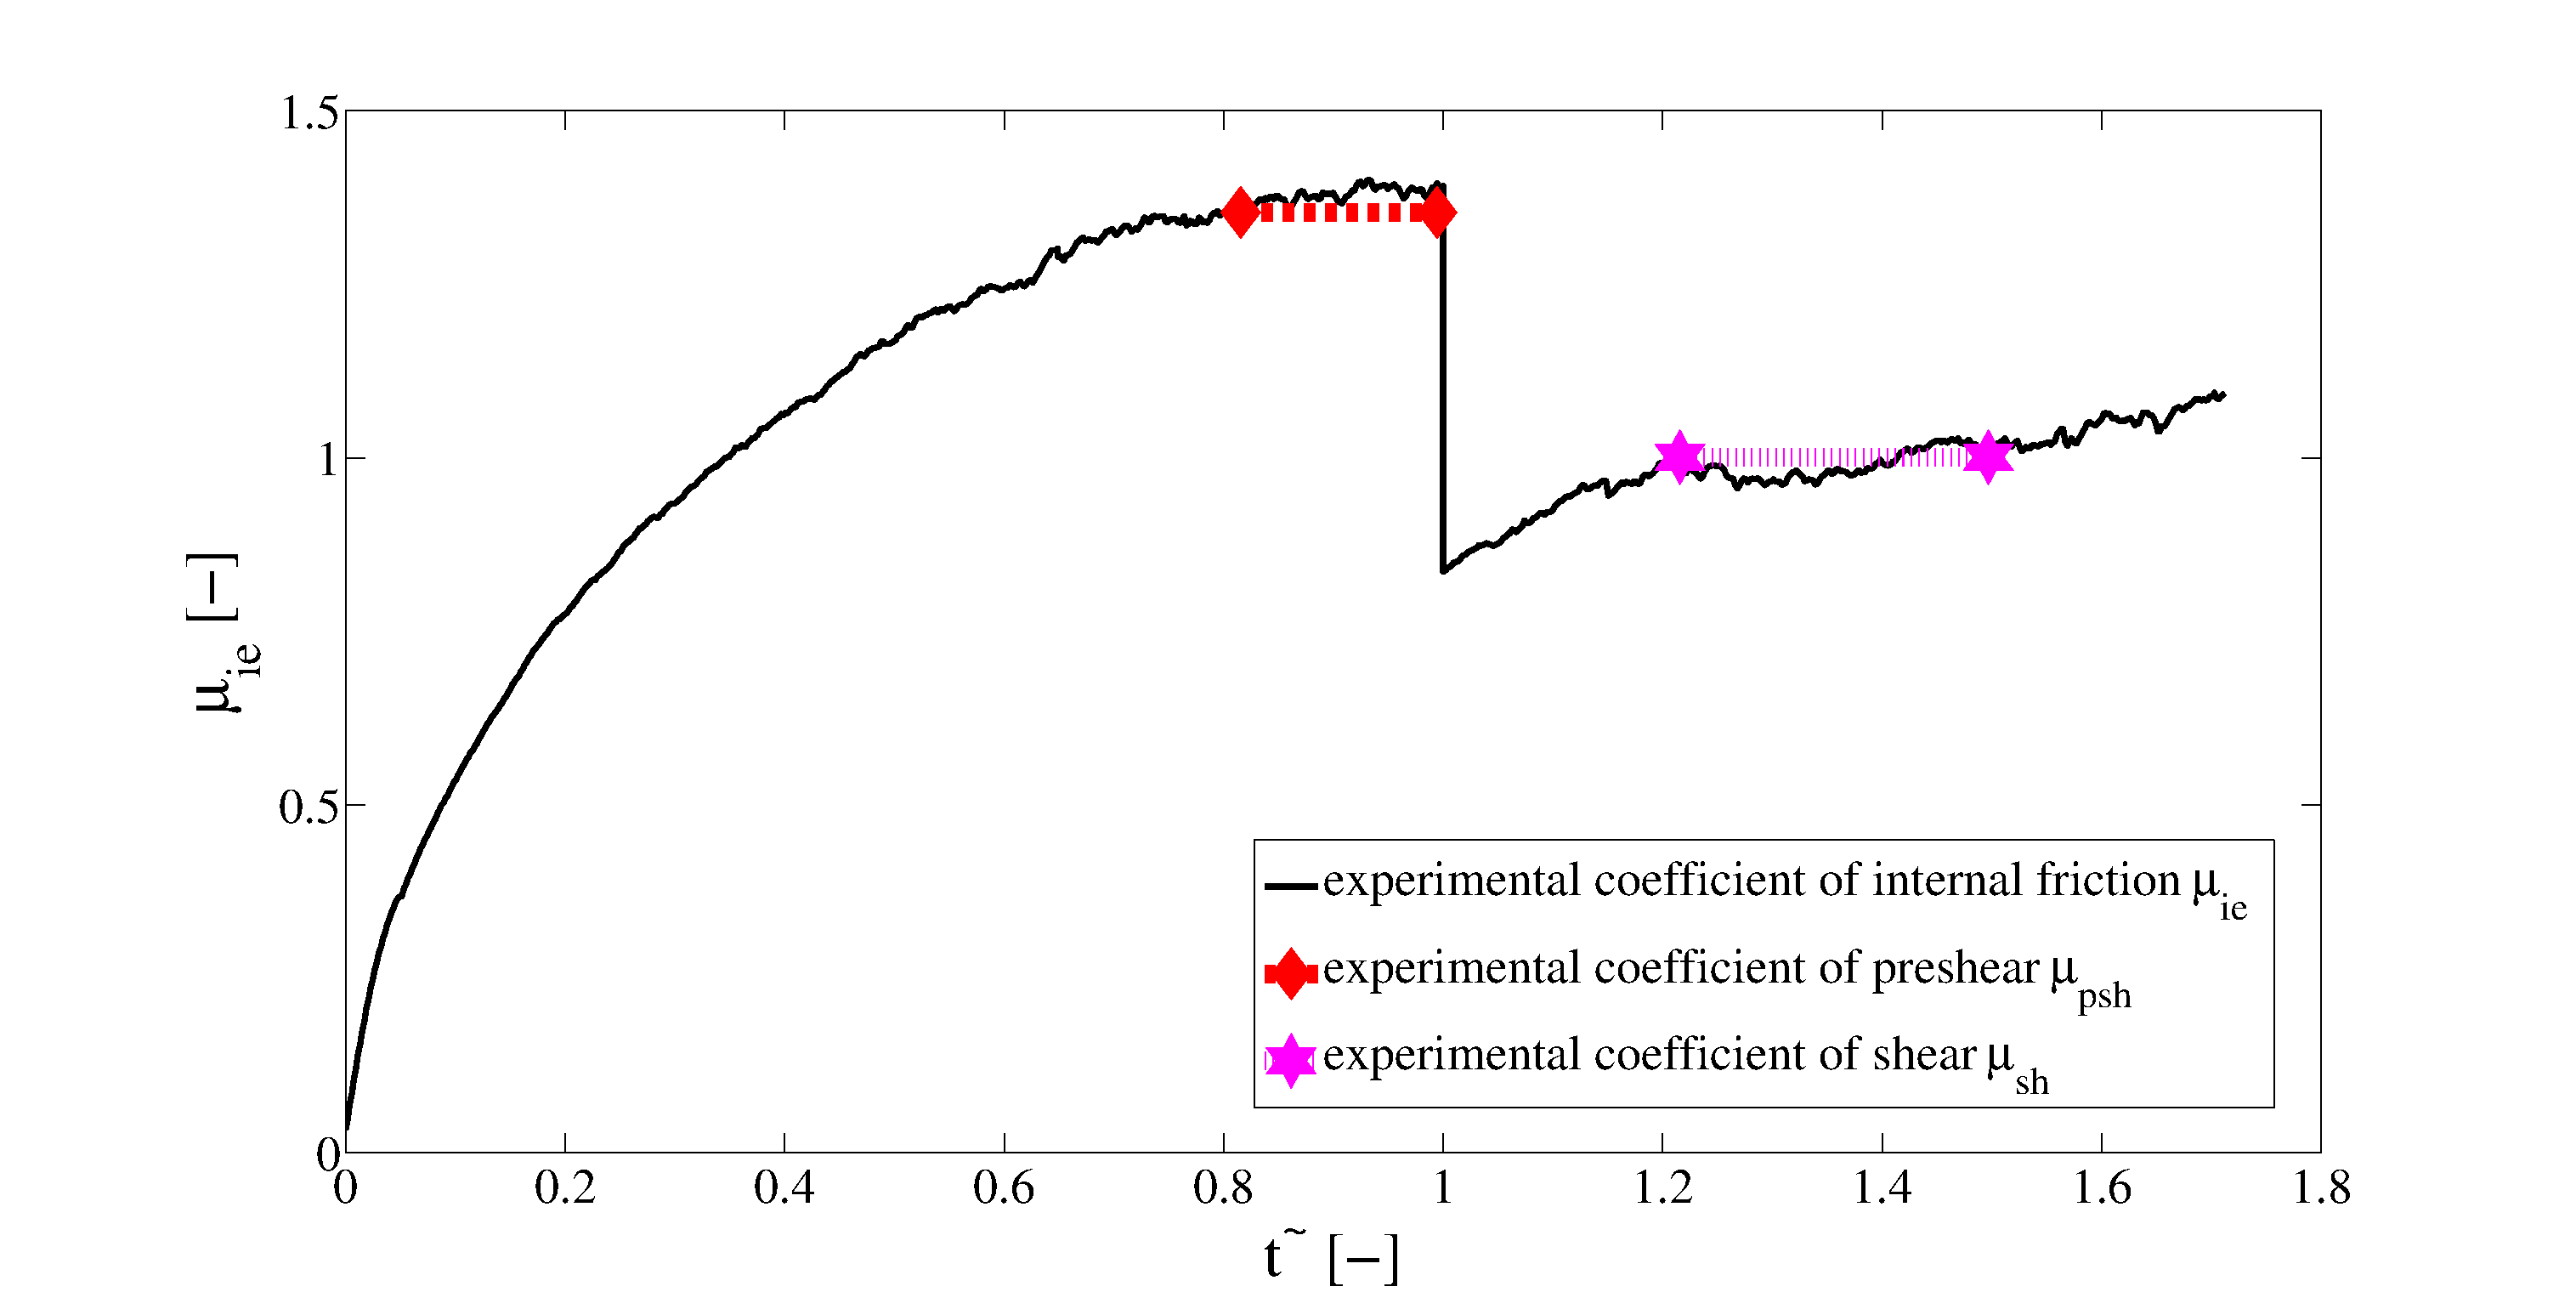
\includegraphics[width=\textwidth]{images/original/20experimental}
        \caption{Experimental shear cell tester stress path - $\sigma_n = 2000
        [Pa]$}
        \label{fig:20experimental} 
    \end{subfigure}\\
        \begin{subfigure}[b]{2cm}
        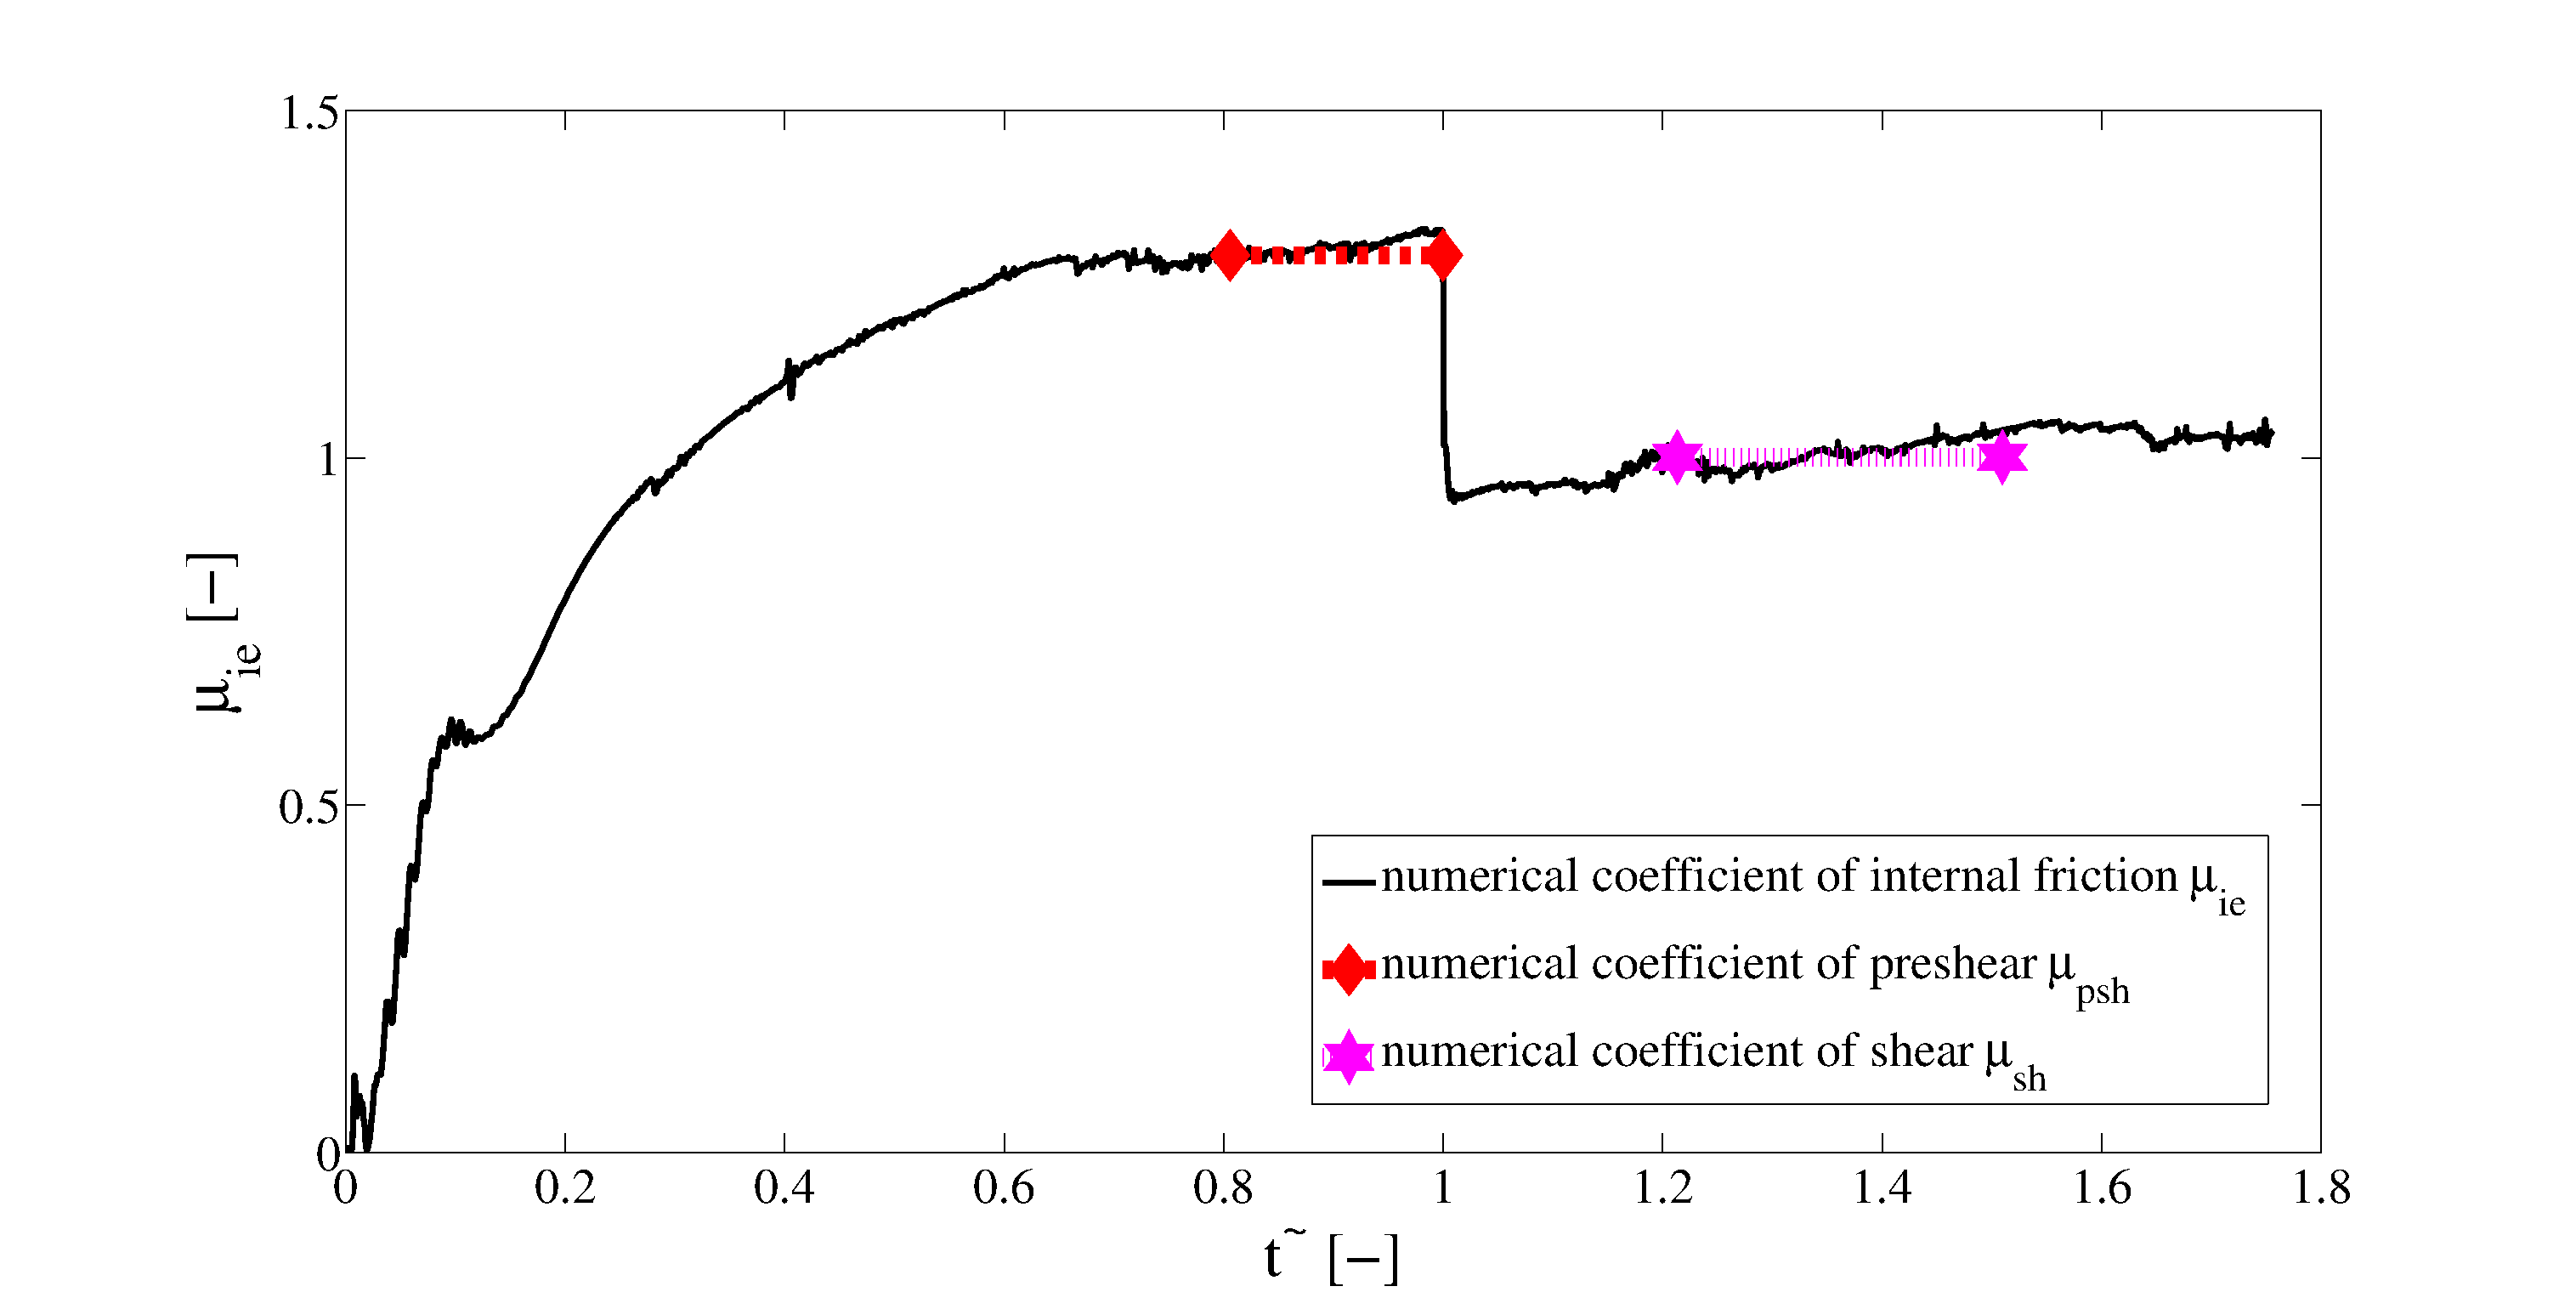
\includegraphics[width=\textwidth]{images/original/21simexample}
        \caption{Numerical shear cell tester stress path - $\sigma_n = 10000
        [Pa]$}
        \label{fig:21simexample} 
    \end{subfigure}
    \caption[Stress path]{Sample of the stress path for
	the Schulze ring shear cell tester, experimental and numerical.
	Time is normalized: $\tilde{t} = t/t_{change}$, where $t_{change}$ is the
	time when the normal stress ($\sigma_n$) is modified during the tests.
	Until $\tilde{t}=1$ the $\sigma_n = 2000 ~[Pa]$ is kept constant. 
	In Fig. \ref{fig:20experimental} at $\tilde{t}~=0.91$
 	a plateau is reached.
	The $\mu_{psh}$ is calculated as average of the $\mu_{ie}$ in this first
	plateau.
	Later, at $\tilde{t}=1$, the $\sigma_n$ is reduced to $80 \%$ of its initial
	value.
	Soon, a second plateau starts.
	As average of $\mu_{ie}$ in this second plateau we obtain $\mu_{sh}$.
	The stress path is in the numerical simulation is comparable to the
	experimental one, especially the plateaux.
	They were clearly relevant because there we collected the numerical bulk
	behaviour representative values. }
    \label{fig:40experimentalsimulation}
\end{figure}

\begin{table}[h]
\centering
\begin{tabular}{ccc}
\hline
    Young's & Poisson's & \acs{deltat}\\
   modulus & ratio & \\
    $[MPa]$ & $[-]$ & [s]\\
    \hline
    $10$    & $0.40$ & $10^{-6}$\\


\hline
\end{tabular}
\caption{DEM fixed input values}
\label{tab:09DEMFixedinputvalues}
\end{table}
\begin{table}[h]
\centering
\begin{tabular}{ccccc}
\hline
    \acs{mus} & \acs{mur} & \acs{CoR} & \acs{rhop} & \acs{dCylDp} \\
    	$[-]$  & $[-]$   & $[-]$   & $[kg/m3]$ & $[-]$ \\
    \hline
    0.4 / 0.6 / 0.8 & 0.4 / 0.6 / 0.8 & 0.5 / 0.7 / 0.9 & 2500 / 3000 / 3500 & 20 / 36 / 38 / 40 \\

\hline
\end{tabular}
\caption[DEM variable input values]{DEM variable input values for training the
Neural Networks}
\label{tab:10DEMVariableinputvalues}
\end{table}
\begin{table}[h]
\centering
\begin{tabular}{lcccc}
\hline
 &  \ac{mus} & \ac{mur} & \ac{CoR} & \ac{rhop}  \\
  &	$[-]$  & $[-]$   & $[-]$   & $[kg/m3]$ \\
          \hline
    range & $[0.1 \ldots 1.0]$ & $[0.1 \ldots 1.0]$ & $[0.5 \ldots 0.9]$ &
    $[2000 \ldots 3500]$     \\
    \# rnd & 100   & 100   & 25    & 25    \\

\hline
\end{tabular}
\caption[DEM random input values]{DEM random input values. Within each range \#
random values are chosen.}
\label{tab:12DEMRandominputvalues}
\end{table}

\subsection{Artificial Neural Networks}
\label{subsec:ann}
We first defined the typology of Artificial Neural Network ($ANN$) we used and
the input we imposed to them, see \ref{sec:appann}.
Our $ANN$ are built with three different layers. 
The input layer has a number of neurons equal to the number of different inputs
of the network, see Fig. \ref{fig:18nnscheme}.
The hidden (or central) layer's number of neurons must be investigated. 
The output layer contains one neuron for the output.
The transfer functions between the first two layers are the tangential sigmoid, 
while between the hidden and central layers are linear.\\
So, we could use the $DEM$ parameter combinations and their corresponding bulk
values to train the $ANN$,
dashed line in Fig. \ref{fig:19methodology}.
Notably, we excluded 15\% of the simulations ($test ~ simulations$),
randomly picked, from the training processes.
We started with all the $DEM$ parameter combinations and their corresponding numerical $\mu_{psh}$ to create 36 $ANN$. 
They differed because they included from five to forty neurons in the hidden
layer.
Later, we controlled the coefficient of determination ($R^2$) between the
$bulk-macro$ behaviours in the output of the $ANN$ and the 15\% $test ~ simulations$, granted uncorrelated. 
So, we could select for $\mu_{psh}$ the $ANN$ with the maximum $R^2$, 
again as suggested by Vaferi et al. \cite{RefWorks:150}, and we noted its number
of neurons.
We repeated the same steps from the $ANN$ creations for $\mu_{sh}$, $\rho_b$ and $AoR$, 
obtaining one trained $ANN$ for each bulk representative value. \\
Notably, $\mu_{psh}$, $\mu_{sh}$ and $\rho_b$ belonged to the shear cell
simulations, so their $ANN$ were handled together. 
We had one cluster with three $ANN$ for the shear cell and one with only one $ANN$
for the $AoR$.
We could then proceed in identifying the valid input parameters, straight line
in Fig. \ref{fig:19methodology}.
Oberkampf et al. \cite{RefWorks:160} suggest to use a Design of Experiments
($DoE$) method to determine the parameters' combinations to be simulated.
They affirm that this approach allows optimizing the computational time with
only an acceptable loss of precision.
Thanks to the speed of the trained $ANN$, we followed a different approach to
maximize the precision of the characterization.
We created random values
in the range and number defined in table \ref{tab:12DEMRandominputvalues}.
Together, the total number of combinations of these random values was $6250000$.
These combinations were then imposed as input and processed by the selected
$ANN$, granting for each three bulk representative parameters for the shear cell and one for the $AoR$. 
\begin{figure}[!htb] 
\centering 
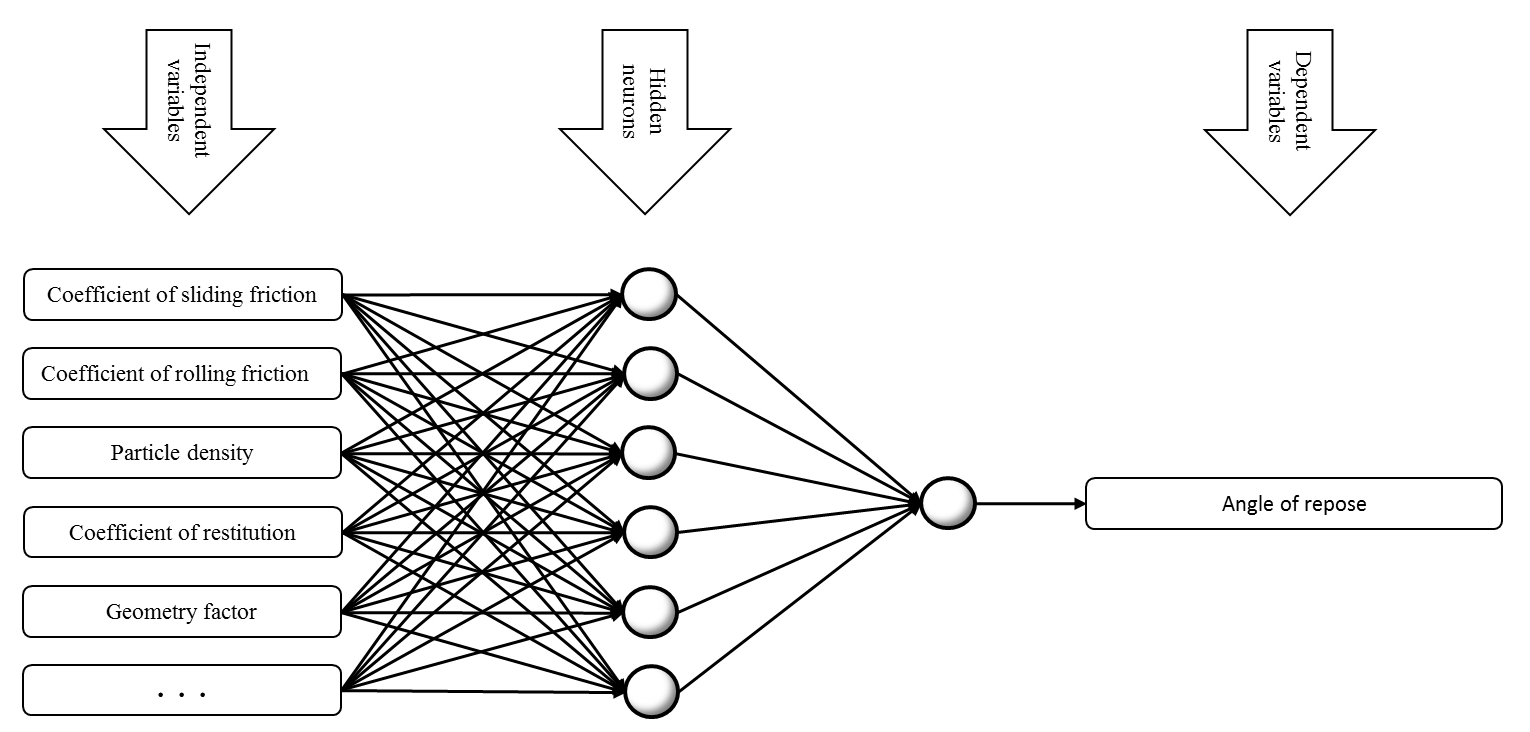
\includegraphics[width=.96\textwidth]{18nnscheme} 
\caption[NN Scheme]{Neural Network ($NN$) Scheme. This is the schematic of how
the Multi Layer Perceptron $NN$ ($MLPNN$) derives one bulk behaviour
dependent variable from the mutually independent simulation variables.}
\label{fig:18nnscheme} 
\end{figure}


% \begin{figure}[htp]
%     \centering
%     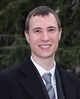
\includegraphics[width=.2\textwidth]{images/vitae/lbenvenuti}
%     \caption{OpenMP, MPI, MPI/OpenMP Hybrid runs of Box in a box testcase on 32
%     cores. The OpenMP-only run suffers from limited memory bandwidth in
%     memory-bound algorithms inside of the Modify section of the code. MPI-only has
%     low averaged runtimes for each section, but a very large Other timing, which
%     hints for a large amount of load-imbalance. Hybrid timings are a bit worse
%     on average, but because of better balancing, processes have lower wait times
%     inside of Other timing.}
% 	\label{fig:boxInBoxComparison}



\subsection{Macroscopic Experiments and Parameter Identification}
\label{subsec:macroscopicexperimentsparameteridentification}
The experimental characterization has been performed as described in
\ref{subsec:srsctexperiment} and \ref{subsec:aorexperiment}. 
We obtained for each of the twelve load conditions of the $SSC$ three values
representative of the bulk behaviour ($\mu_{psh}$, $\mu_{sh}$ and $\rho_b$).
Furthermore, to recreate the repose angle observed in a pile of the real material, 
we performed two angle of repose ($AoR$) tests, as the $AoR$ was the fourth
behaviour value. 

Later, we confronted the $ANN$ and experimental bulk behaviours for the twelve shear cell load conditions. 
If in a $DEM-parameter$ combination all the three bulk representative parameters differed less 
than 5\% from the corresponding experiments, see Eq. \ref{eq:check2}:
\begin{equation}
 \begin{cases}
\text{if } & \lvert{1-\frac{\mu_{psh,num}}{\mu_{psh,exp}}}\rvert < 5\%  ,\\
\text{and if } & \lvert{1-\frac{\mu_{sh,num}}{\mu_{sh,exp}}}\rvert < 5\% , \\ 
\text{and if } & \lvert{1-\frac{\rho_{p,num}}{\rho_{p,exp}}}\rvert < 5\% ,\\ 
\end{cases}
 \label{eq:check2}
\end{equation}
then the combination was marked. The marked combinations were handled by the
$AoR$ $ANN$, and then confronted with the experiment.
Were branded as valid only those that differed less than $5\%$ also in this
comparison (Eq. \ref{eq:checkaor}):
\begin{equation}
\text{if} ~~~~~~ \lvert{1-\frac{AoR_{num}}{AoR_{exp}}}\rvert < 5\% .
\label{eq:checkaor}
\end{equation}
%************************************************
Further, to prove the system validity, we tested the marked combinations by
modifying the experimental bulk behaviour representative values of the shear cell. 
We artificially decreased or increased $\mu_{psh}$ and $\mu_{sh}$ by a product
coefficient ($P$), e.g. Eq. \ref{eq:pcoeff}:
\begin{equation}
\label{eq:pcoeff}
\mu_{psh, new} = \mu_{psh, old} \cdot P .
\end{equation}


% \subsection{ Methodology}
% \label{subsec:parameteridentificationmethodology}
